% !TeX root = markov.tex

%%%%%%%%%%%%%%%%%%%%%%%%%%%%%%%%%%%%%%%%%%%%%%%%%%%%%%%%%%%%%%%%

\documentclass[11pt,a4paper]{article}

\usepackage{mathpazo}
\usepackage{microtype}
\usepackage{url}
\usepackage{graphicx}

% TikZ package
\usepackage{tikz}
\usetikzlibrary{arrows.meta}
\usetikzlibrary{positioning}
\usetikzlibrary{automata}
\tikzset {>=Stealth}

% Displaystyle for fractions and combinations
\newcommand*{\disfrac}[2]{\displaystyle\frac{#1}{#2}}
\newcommand*{\dischoose}[2]{\displaystyle{#1 \choose #2}}
\newcommand*{\sm}[1]{$\scriptstyle #1$}

% Change LaTeX defaults for figures
\renewcommand{\topfraction}{0.9}
\renewcommand{\bottomfraction}{0.8}
\setcounter{topnumber}{1}
\setcounter{bottomnumber}{2}
\setcounter{totalnumber}{3}
\renewcommand{\textfraction}{0.07}
\renewcommand{\floatpagefraction}{0.7}

% Layout
\textwidth=150mm
\textheight=225mm
\topmargin=0pt
\headheight=11pt
\oddsidemargin=1em
\evensidemargin=0mm
\headsep=0pt
\parindent=0pt
\renewcommand{\baselinestretch}{1.1}
\setlength{\parskip}{0.3\baselineskip plus 1pt minus 1pt}

\begin{document}

%%%%%%%%%%%%%%%%%%%%%%%%%%%%%%%%%%%%%%%%%%%%%%%%%%%%%%%%%%%%%%%%%%%%%

\thispagestyle{empty}

\begin{center}
\textbf{\LARGE Markov Chain Simulations}

\bigskip
\bigskip
\bigskip

\textbf{\Large Moti Ben-Ari}

\bigskip

\url{http://www.weizmann.ac.il/sci-tea/benari/}

\bigskip
\bigskip
\bigskip

\today

\end{center}

\vfill

\begin{center}
\copyright{} Moti Ben-Ari $2023$
 \end{center}
 
\begin{small}
This work is licensed under Attribution-ShareAlike 4.0 International. To view a copy of this license, visit \url{http://creativecommons.org/licenses/by-sa/4.0/}.
\end{small}
\newpage

\tableofcontents

\newpage

%%%%%%%%%%%%%%%%%%%%%%%%%%%%%%%%%%%%%%%%%%%%%%%%%%%%%%%%%%%%%%%%%%%%%


\section{Introduction}

Simulations are an excellent way of understanding probability, especially the behavior of processes of long duration. Simulation programs enable the user to perform experiments by varying the parameters of problems and analyzing. The simulations in this archive are of processes known as \emph{Markov chains}, where the next state of the system depends only on the current state and not on the history of how the process got to the current state. 

The following problems are simulated: gambler's ruin, the ballot box, one-, two- and three-dimensional random walk and random walk in a circle, the Ehrenfest model, the two-state process and transversing a maze.

A knowledge of probability is assumed at the level of the first few chapters of \cite{BW,ross}. The problems and their theoretical solutions are from the works cited in the references.

\nocite{*}

The programs are written in the Python 3 language and use the \verb+matplotlib+ library to generate the graphs. You need to install Python (\url{https://www.python.org/downloads/}) although a knowledge of Python programming is not necessary to run the simulations.

Parameters directly related to the problems, such as the probability of success, can be modified interactively. Others, related to the simulation, such as the number of steps in a simulation, are defined in a file \verb+configuration.py+. The code that uses \verb+matplotlib+ also appears in a separate file.

%%%%%%%%%%%%%%%%%%%%%%%%%%%%%%%%%%%%%%%%%%%%%%%%%%%%%%%%%%%%%%%%%%%%%

\section{Gambler's ruin}\label{s.gamblers}

Two players $A$ and $B$ compete in a contest. There is an initial finite capital of $n$ units: $A$ has $i$ and $B$ has $n-i$. They repeatedly play a game where the probability that $A$ wins is $p$ and the probability that $B$ wins is $q=1-p$. The loser gives one unit to the winner. When one player has all $n$ units the contest is terminated and that player is declared the winner.
\begin{center}
\begin{tikzpicture}[scale=1.2]
\draw (0,0) node[above left] {$A$} -- 
      (10,0) node[above right] {$B$};
\foreach \x in {0,1,2,3,4,5,6,7,8,9,10} {
  \draw (\x,0) -- +(0,4pt);
  \node at (\x,-10pt) { $\x$ };
}
\node at (4,-9mm) {$i$};
\node at (10,-9mm) {$n$};
\draw[fill] (4,7mm) circle[radius=1pt];
\draw[->] (4,7mm) -- node[above] {$q$} +(-1,0);
\draw[->] (4,7mm) -- node[above] {$p$} +(1,0);
\end{tikzpicture}
\end{center}
\begin{itemize}
\item Given initial parameters $(p, n, i)$, what is the probability that $A$ wins?
\item What is the expected duration of the game?
\end{itemize}

Given $(p,n,i)$ the probability that $A$ wins the contest is:
\[
P_A(p, n, i) = \left(\frac{1-r^{i}}{1-r^n}\right)\,,
\]
where $r=q/p$. By symmetry, the probability that $B$ wins is:
\[
P_B(p, n, i) = \left(\frac{1-(1/r)^{n-i}}{1-(1/r)^{n}}\right)\,.
\]

For $p\neq 1/2$ the expected duration of the contest is:
\[
E_{\mathit{duration}}(p,n,i)=\frac{1}{q-p}\left(i-n
\frac{1-r^k}{1-r^n}\right)\,,
\]
while for $p=1/2$ the expected duration is:
\[
E_{\mathit{duration}}(p,n,i)=i(n-1)\,.
\]
Of course the duration does not depend on which player wins. If $A$ wins, the contest terminates for $B$ and conversely.

You can run a simulation more than once with the saved parameters, enter new parameters, or run a sequence of simulations for a range of probabilities or initial values. Here is one output:
\begin{verbatim}
Probability = 0.45, capital = 20, initial = 8
Wins = 789, losses = 9211, limits exceeded = 0
Proportion of wins     = 0.0789
Probability of winning = 0.0732
Average duration  = 65
Expected duration = 65
\end{verbatim}
A graph of the proportion of wins and the histogram of the durations are shown in Figures~\ref{f.gambler-hist1}, \ref{f.gambler-hist2}. The vertical lines in the histograms are the average durations.

\begin{figure}
\begin{center}
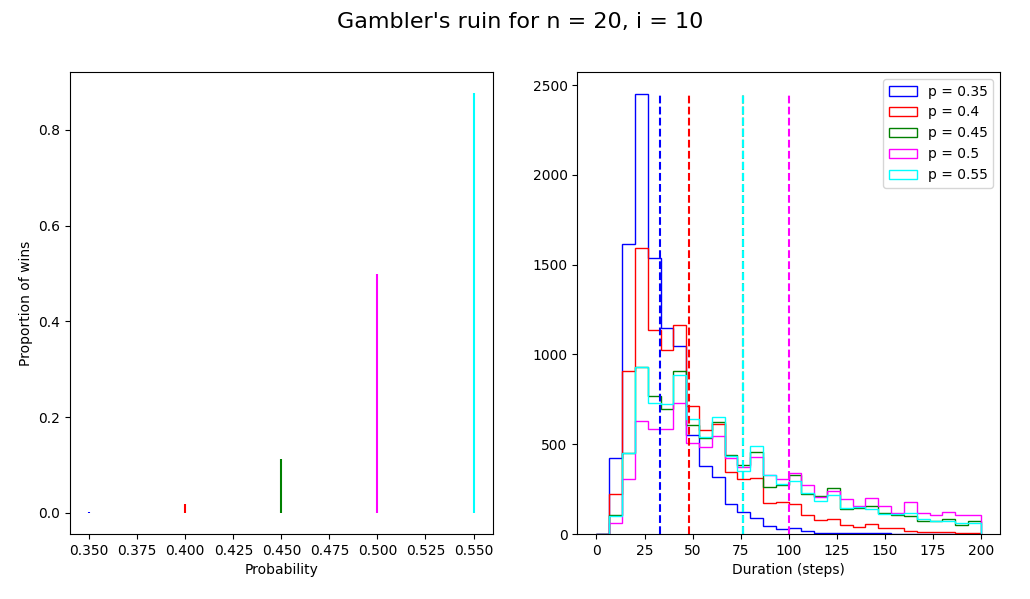
\includegraphics[width=\textwidth]{gamblers-ruin-01}
\caption{Proportion of wins and histogram for $n=20, i=10$ and multiple probabilities}\label{f.gambler-hist1}
\end{center}
\end{figure}

\begin{figure}
\begin{center}
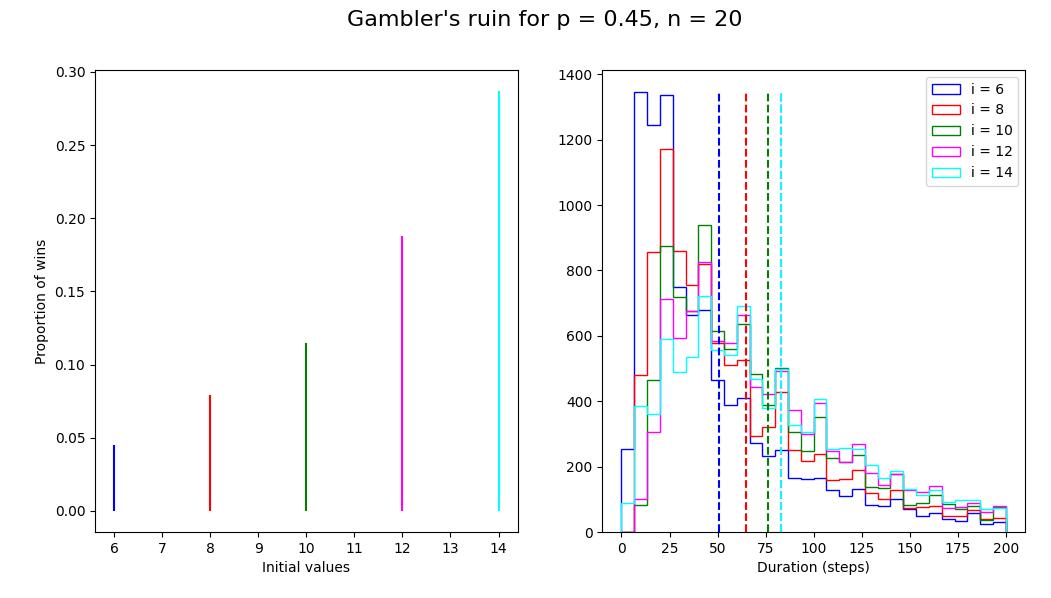
\includegraphics[width=\textwidth]{gamblers-ruin-02}
\caption{Proportion of wins and histogram for $p=0.45, n=20$ and multiple initial values}\label{f.gambler-hist2}
\end{center}
\end{figure}

%%%%%%%%%%%%%%%%%%%%%%%%%%%%%%%%%%%%%%%%%%%%%%%%%%%%%%%%%%%%%%%%%%%%%

\section{The ballot box}\label{s.ballot}

In an election there are two candidates $A$ and $B$.  $A$ receives $a$ votes and $B$ receives $b$ votes where $a>b$. The votes are counted one-by-one and the running totals $(a_i,b_i), 1\leq i \leq a+b$ are updated as each vote is counted. What is the probability that $a_i>b_i$ always holds?

The probability is:
\[
P(A \;\textrm{is always leading}) = \disfrac{a-b}{a+b}\,.
\]
The result of a simulation is:
\begin{verbatim}
For a = 20, b = 18:
Probability of A always leading = 0.0526
Proportion  of A always leading = 0.0510
\end{verbatim}
A graph of the probability and the proportion of simulations that $A$ is always leading is shown in Figure~\ref{f.ballot-01}. As $b$ gets closer to $a$ the probability decreases since more and more votes for $B$ are available to be counted.
\begin{figure}
\begin{center}
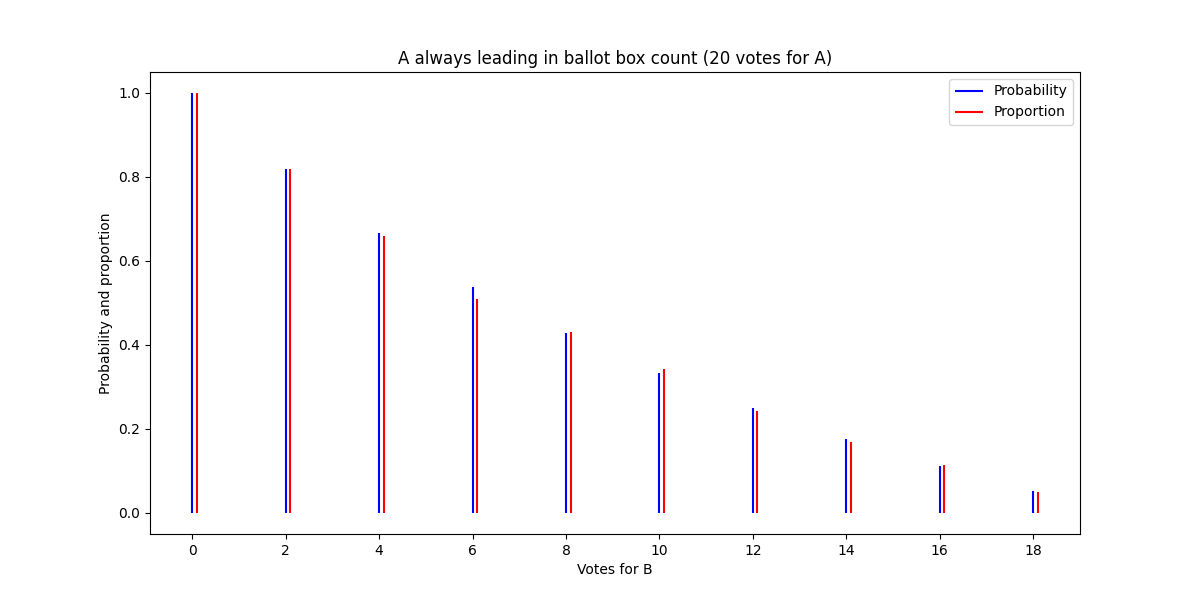
\includegraphics[width=\textwidth]{ballot-01}
\caption{Probability and proportion of $A$ always leading}\label{f.ballot-01}
\end{center}
\end{figure}

%%%%%%%%%%%%%%%%%%%%%%%%%%%%%%%%%%%%%%%%%%%%%%%%%%%%%%%%%%%%%%%%%%%%%

\section{Random walk}\label{s.walk}

\subsection{One-dimensional random walk}

A particle is placed at the origin of the $x$-axis. It repeatedly takes steps: right with probability $p$ and left with probability $q=1-p$.
\begin{center}
\begin{tikzpicture}[scale=1.2]
\draw[<->] (-6,0) -- (6,0);
\foreach \x in {-5,-4,-3,-2,-1,0,1,2,3,4,5} {
  \draw (\x,0) -- +(0,4pt);
  \node at (\x,-10pt) { $\x$ };
}
\node at (-6,-10pt) { $\cdots$ };
\node at (6,-10pt) { $\cdots$ };
\draw[fill] (0,7mm) circle[radius=1pt];
\draw[->] (0,7mm) -- node[above] {$q$} +(-1,0);
\draw[->] (0,7mm) -- node[above] {$p$} +(1,0);
\end{tikzpicture}
\end{center}
\begin{itemize}
\item What is the probability that the particle will return to the origin?
\item What is the expected duration until the particle returns to the origin?
\end{itemize}

By symmetry let the first step be to the right. The particle can only return to the origin after an even number of steps. Assume that $p=1/2$. Let $S_{2m}$ be the position of the particle after $2m$ steps. Then:
\[
P(S_{2m}=0) = \dischoose{2m}{m}\disfrac{1}{2^{2m}}\,,
\]
which by Stirling's formula is approximately equal to $1/\sqrt{\pi m}$. It can now be proved that the probability of a return to the origin is $1$.

For $p\leq 1/2$, $P_{\mathit{origin}}$, the probability of a return to the origin, is $1$ and for $p\geq 1/2$ the probability is (Figure~\ref{f.walk1}):
\[
P_{\mathit{origin}} = \disfrac{q}{p}=\disfrac{1-p}{p}\,.
\]
\begin{figure}
\begin{center}
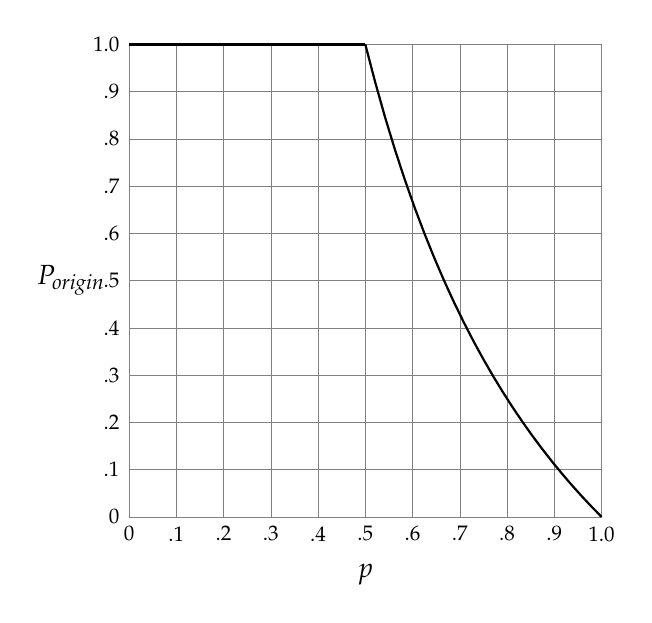
\begin{tikzpicture}[scale=6]
\draw[help lines,step=.1] (0,0) grid (1,1);
\foreach \x in {0,.1,.2,.3,.4,.5,.6,.7,.8,.9,1.0}
  \node[below] at (\x,0) {$\scriptstyle \x$};
\foreach \y in {0,.1,.2,.3,.4,.5,.6,.7,.8,.9,1.0}
  \node[left] at (0,\y) {$\scriptstyle \y$};
\draw[domain=0:.5,thick] plot (\x,1);
\draw[domain=.5:1,thick] plot (\x,{(1-\x)/\x});
\node at (.5,-3.5pt) {$p$};
\node at (-3.5pt,.5) {$P_{\mathit{origin}}$};
\end{tikzpicture}
\caption{Graph of $P_{\mathit{origin}}$}\label{f.walk1}
\end{center}
\end{figure}

$E_{\mathit{origin}}$, the expected duration until the first return to the origin, is infinite for $p\geq 1/2$ while for $p<1/2$ it is:
\[
E_{\mathit{origin}}=\disfrac{1}{q-p}=\disfrac{1}{1-2p}\,.
\]

You can run a simulation more than once with the saved parameters, enter new parameters, or run a sequence of simulations for a range of probabilities or limits. Here is one output:
\begin{verbatim}
Probability = 0.50, step limit   = 1000
Proportion returning to origin   = 0.977
Probability of return to origin  = 1.000
Proportion reaching limit        = 0.023
Mean duration (steps)            = 49
Expected duration (steps)        = infinity
\end{verbatim}
The proportion of wins in the simulation are very close to the theoretical probability, but the mean duration is far from infinite because the step limit was too small.  The proportion of wins and the mean durations are shown in Figures~\ref{f.random-walk-01} and \ref{f.random-walk-02}.
\begin{figure}
\begin{center}
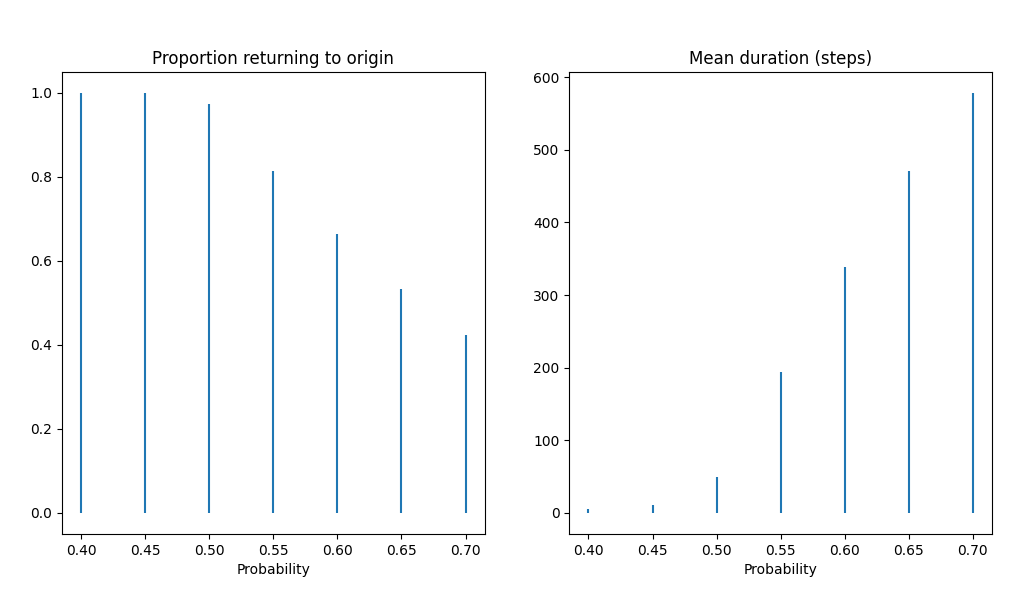
\includegraphics[width=\textwidth]{random-walk-01}
\caption{Proportion of returns to origin and and mean durations for multiple probabilities}\label{f.random-walk-01}
\end{center}
\end{figure}
\begin{figure}
\begin{center}
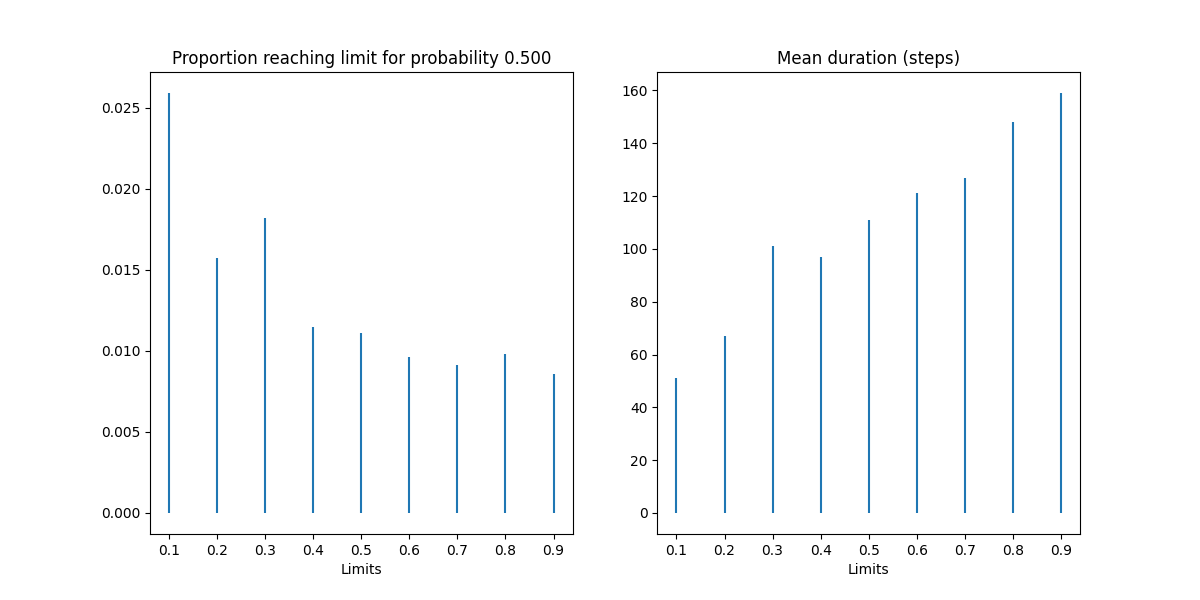
\includegraphics[width=\textwidth]{random-walk-02}
\caption{Proportion of returns to origin and mean durations for multiple limits}\label{f.random-walk-02}
\end{center}
\end{figure}

\subsection{Two-dimensional random walk}

In a two-dimensional random walk a step of the particle consists of one step left or right on the $x$-axis with probability $1/2$ and simultaneously one step up or down on the $y$-axis also with probability $1/2$ (Figure~\ref{f.2d-random-walk}).

\begin{figure}
\begin{center}
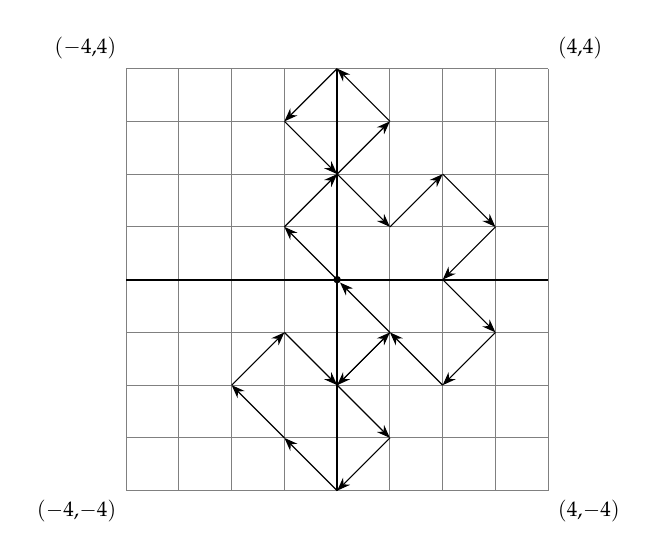
\begin{tikzpicture}[scale=.67]
\draw[color=gray] (-4,-4) grid (4,4);
\draw[thick] (-4,0) -- (4,0);
\draw[thick] (0,-4) -- (0,4);
\node[below left] at (-4,-4) {$\scriptstyle (-4,-4)$};
\node[below right] at (4,-4) {$\scriptstyle (4,-4)$};
\node[above left] at (-4,4) {$\scriptstyle (-4,4)$};
\node[above right] at (4,4) {$\scriptstyle (4,4)$};
\fill (0,0) circle[radius=2pt];
\draw[->] (0,0)  -- (-1,1);
\draw[->] (-1,1) -- (0,2);
\draw[->] (0,2)  -- (1,3);
\draw[->] (1,3)  -- (0,4);
\draw[->] (0,4)  -- (-1,3);
\draw[->] (-1,3) -- (0,2);
\draw[->] (0,2)  -- (1,1);
\draw[->] (1,1)  -- (2,2);
\draw[->] (2,2)  -- (3,1);
\draw[->] (3,1)  -- (2,0);
\draw[->] (2,0)  -- (3,-1);
\draw[->] (3,-1) -- (2,-2);
\draw[->] (2,-2) -- (1,-1);
\draw[->] (1,-1) -- (0,-2);
\draw[->] (0,-2) -- (1,-3);
\draw[->] (1,-3) -- (0,-4);
\draw[->] (0,-4) -- (-1,-3);
\draw[->] (-1,-3)-- (-2,-2);
\draw[->] (-2,-2)-- (-1,-1);
\draw[->] (-1,-1)-- (0,-2);
\draw[->] (0,-2) -- (1,-1);
\draw[->] (1,-1) -- (.055,-.055);
\end{tikzpicture}
\end{center}
\caption{A $22$-step two-dimensional random walk}\label{f.2d-random-walk}
\end{figure}
The probability $1$ the particle will return to the origin but the expected duration is infinite! Therefore, when you run the simulation with any reasonable limit on the number of steps, the proportion of returns to the origin will be much less than $1$ and the mean duration will be quite large:
\begin{verbatim}
Limit                            = 100000
Proportion returning to origin   = 0.777
Proportion reaching limit        = 0.223
Mean duration (steps)            = 24133
\end{verbatim}
Figure~\ref{f.random-walk-2D} shows the proportion of returns to the origin and the mean durations for a range of fractions of the limit.

\begin{figure}
\begin{center}
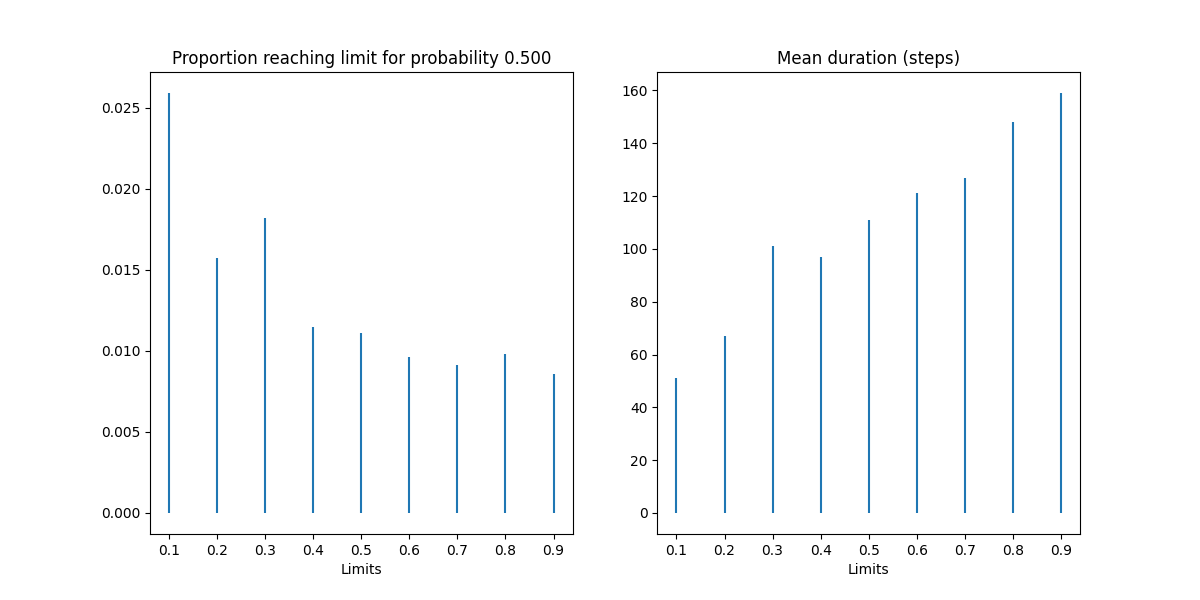
\includegraphics[width=\textwidth]{random-walk-02}
\caption{Proportion of returns to origin and and mean durations for multiple limits}\label{f.random-walk-2D}
\end{center}
\end{figure}

\subsection{Three-dimensional random walk}

The three-dimensional random walk adds a simultaneous step along the $z$-axis with probability $1/2$. The probability of a return to the origin is only $0.2379$ so the simulations will show a large number of simulations reaching the limit:

\begin{verbatim}
Limit                            = 100000
Proportion returning to origin   = 0.370
Proportion reaching limit        = 0.630
Mean duration (steps)            = 63518
\end{verbatim}

\subsection{Random walk in a circle}

Consider a circle with $n$ equally-spaced points around its circumference (Figure~\ref{f.random-walk-circle}). A random walk starts at point $0$ and proceeds to the next point or the previous point both with probability $1/2$.

\begin{figure}
\begin{center}
\begin{tikzpicture}
\draw (0,0) circle[radius=2.5];
\foreach \angle/\label in
  {0/3,30/2,60/1,90/0,120/11,150/10,180/9,210/8,240/7,270/6,300/5,330/4} {
    \fill (\angle:2.5) circle[radius=1.5pt];
    \node at (\angle:2.8) {$\scriptstyle\label$};
}
\node at (334:3.2) {$k$};
\end{tikzpicture}
\end{center}
\caption{Random walk in a circle}\label{f.random-walk-circle}
\end{figure}

\begin{itemize}
\item With probability $1$ the all points will be visited.
\item With probability $1/n$ a designated point $k$ will be the last point visited.
\end{itemize}

The random walk will eventually visit all points, but it make take a very large number of steps. (Try to run the simulation for $100$ points!) Here is an output:
\begin{verbatim}
For 50 points, 1000 simulations, at most 3000 steps:
  Designated point visited 22 times
    Probability = 0.020, proportion = 0.022
  Did not visit all points 26 times
\end{verbatim}
The histogram of steps visited is shown Figure~\ref{f.random-walk-circle-histogram}. 
\begin{figure}
\begin{center}
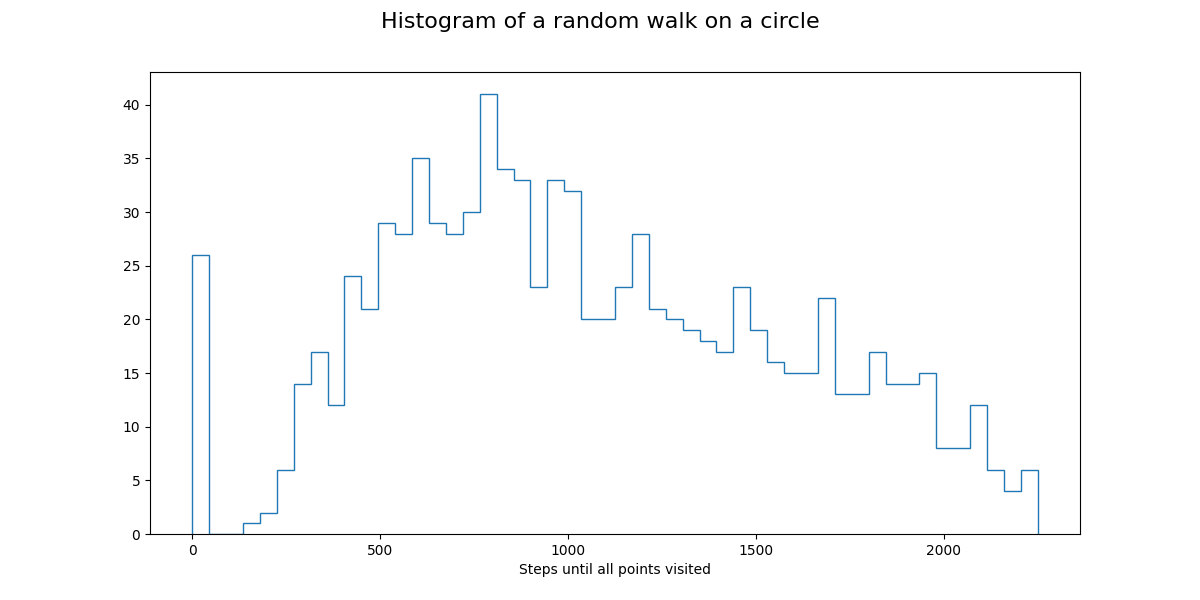
\includegraphics[width=\textwidth]{random-walk-circle}
\caption{Histogram of steps until all points are visited}\label{f.random-walk-circle-histogram}
\end{center}
\end{figure}


%%%%%%%%%%%%%%%%%%%%%%%%%%%%%%%%%%%%%%%%%%%%%%%%%%%%%%%%%%%%%%%%%%%%%

\section{The Ehrenfest model}\label{s.ehrenfest}

The Ehrenfest model models the diffusion of particles between two containers. In the following diagram there are $4$ particles in the left container and $6$ in the right container.
\begin{center}
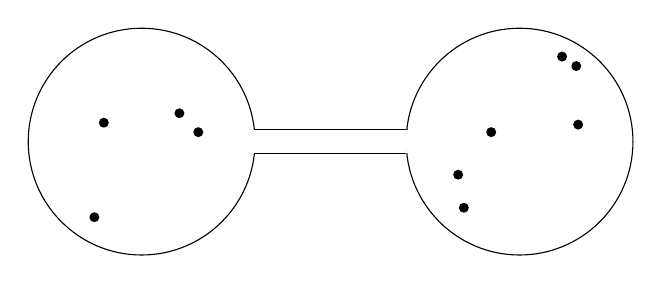
\begin{tikzpicture}[scale=1.2]
\draw (0,0) node {} circle[radius=1.2];
\draw[white,thick] (-6:1.2) arc(-6:6:1.2);
\draw (-6:1.2) -- +(1.63,0);
\draw (6:1.2) -- +(1.63,0);
\fill (-.4,.2) circle[radius=1.5pt];
\fill (.4,.3) circle[radius=1.5pt];
\fill (-.5,-.8) circle[radius=1.5pt];
\fill (.6,.1) circle[radius=1.5pt];
\begin{scope}[xshift=4cm]
\draw (0,0) node {} circle[radius=1.2];
\draw[white,thick] (174:1.2) arc(174:186:1.2);
\fill (-.3,.1) circle[radius=1.5pt];
\fill (.45,.9) circle[radius=1.5pt];
\fill (-.65,-.35) circle[radius=1.5pt];
\fill (.62,.18) circle[radius=1.5pt];
\fill (-.59,-.7) circle[radius=1.5pt];
\fill (.6,.8) circle[radius=1.5pt];
\end{scope}
\end{tikzpicture}
\end{center}
Repeatedly choose a particle at random with uniform distribution and move it to the other container. If there are $i$ particles in the left container then the probability of choosing a particle from the left container is $i/n$ and the probability of choosing a particle from the right container is $(n-i)/n$. If one container is empty the next particle must be chosen from the other container. 
\begin{center}
\begin{tikzpicture}[scale=1.2]
\draw (0,0) node[above left] {$A$} -- 
      (10,0) node[above right] {$B$};
\foreach \x in {0,1,2,3,4,5,6,7,8,9,10} {
  \draw (\x,0) -- +(0,4pt);
  \node at (\x,-10pt) { $\x$ };
}
\node at (4,-9mm) {$i$};
\node at (10,-9mm) {$n$};
\draw[fill] (4,7mm) circle[radius=1pt];
\draw[->] (4,7mm) -- node[above,xshift=-8pt] {$(n-i)/n$} +(-1,0);
\draw[->] (4,7mm) -- node[above,xshift=2pt] {$i/n$} +(1,0);
\draw[->] (0,7mm) -- node[above] {$1$} +(1,0);
\draw[<-] (9,7mm) -- node[above] {$1$} +(1,0);
\end{tikzpicture}
\end{center}
The problem is similar to the gambler's ruin except that the process never ends and the probability of a left or right step changes with each step.

The process is a Markov chain which eventually reaches a \emph{stationary distribution}:
\[
s_i=\dischoose{n}{i}\left(\frac{1}{n}\right)^n\,,
\]
where $s_i$ is the proportion of time that the particle is at the $i$'th position.

Here is an output of the simulation:
\begin{verbatim}
Total particles in urns = 10
Theoretical stationary distribution
[0.001 0.01  0.044 0.117 0.205 0.246 0.205 0.117 0.044 0.01  0.001]
Simulation stationary distribution
[0.001 0.009 0.044 0.12  0.208 0.243 0.205 0.121 0.042 0.008 0.001]
\end{verbatim}
A graph of these distributions is shown in Figure~\ref{f.ehrenfest1}; the theoretical distribution and the result of simulation are so close together that the lines are slightly offset.

\begin{figure}
\begin{center}
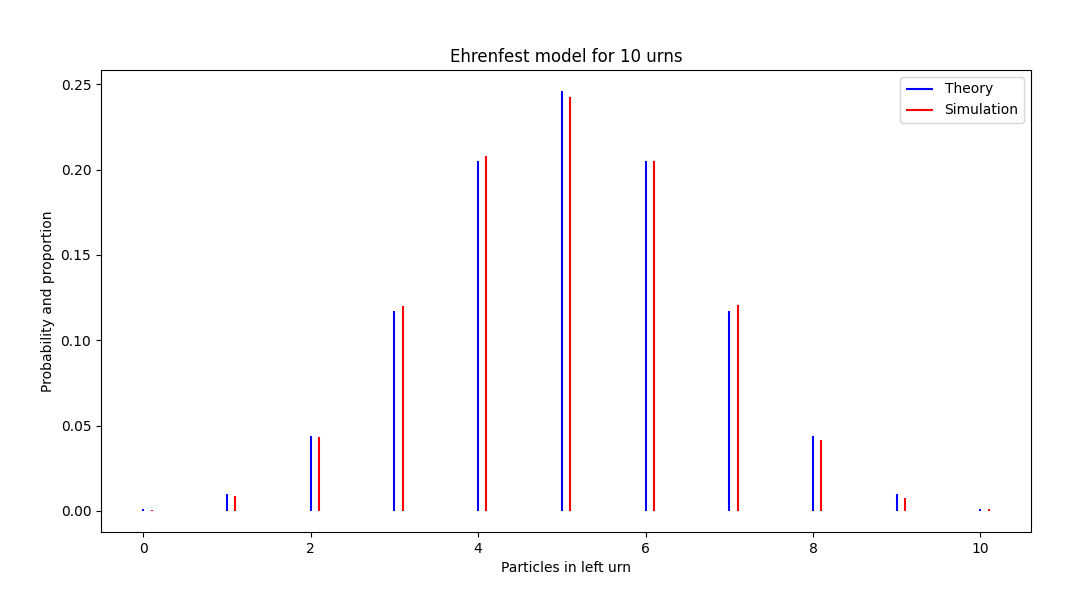
\includegraphics[width=\textwidth]{ehrenfest-01}
\caption{Stationary distribution for the Ehrenfest model}\label{f.ehrenfest1}
\end{center}
\end{figure}

%%%%%%%%%%%%%%%%%%%%%%%%%%%%%%%%%%%%%%%%%%%%%%%%%%%%%%%%%%%%%%%%%%%%%

\section{The two-state process}\label{s.two-state}

The two-state process is similar to the Ehrenfest model in that the probabilities at each step are different and we are interested in the stationary probability distribution of the unbounded process. There are two states $A,B$. In state $A$ the process transitions to $B$  with probability $a$ and remains in $A$ with probability $1-a$. Similarly, the probability of a transition from $B$ to $A$ is $b$ and the probability of remaining in $B$ is $1-b$.
\begin{center}
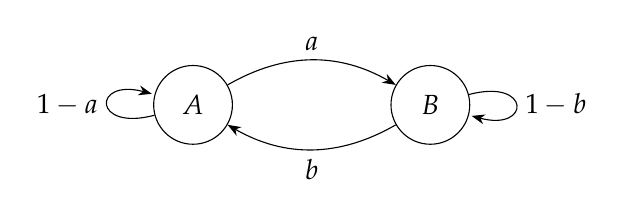
\begin{tikzpicture}[->,node distance = 6mm and 2cm]
\node[draw,circle,minimum size=10mm] (A) {$A$};
\node[draw,circle,minimum size=10mm] (B) [right=of A] {$B$};
\draw (A) edge[bend left] node[above] {$a$} (B);
\draw (B) edge[bend left] node[below] {$b$} (A);
\draw (A) edge [loop left] node {$1-a$} (A);
\draw (B) edge [loop right] node {$1-b$} (B);
\end{tikzpicture}
\end{center}
The stationary distribution, that is, the proportion of visits to $A$ and to $B$ is:
\[
\left[\frac{b}{a+b}, \frac{a}{a+b}\right]\,.
\]
Here is an output of a simulation:
\begin{verbatim}
Probabilities:  a = 0.500, b = 0.333
Theoretical stationary distribution: A = 0.400, B = 0.600
Simulation  stationary distribution: A = 0.402, B = 0.598
\end{verbatim}
When $a+b=1$ the probability of being at $A$ is $b$ and the probability of being at $B$ is $a$:
\begin{verbatim}
Probabilities:  a = 0.333, b = 0.667
Theoretical stationary distribution: A = 0.667, B = 0.333
Simulation  stationary distribution: A = 0.674, B = 0.326
\end{verbatim}
You can enter a required proportion $p$ of visits to $B$ and any probability $0<a<p$. The proportion will be achieved for:
\[
b = \frac{a(1-p)}{p}\,,
\]
as shown in the following simulation where we entered $p=0.8, a=0.6$:
\begin{verbatim}
Probabilities:  a = 0.600, b = 0.150, proportion = 0.800
Theoretical stationary distribution: A = 0.200, B = 0.800
Simulation  stationary distribution: A = 0.194, B = 0.806
\end{verbatim}

%%%%%%%%%%%%%%%%%%%%%%%%%%%%%%%%%%%%%%%%%%%%%%%%%%%%%%%%%%%%%%%%%%%%%

\section{A maze}\label{maze}

Given the Markov chain shown in the following diagram, simulate the average number of steps until the first return to state $i$ starting in state $j$.
\begin{center}
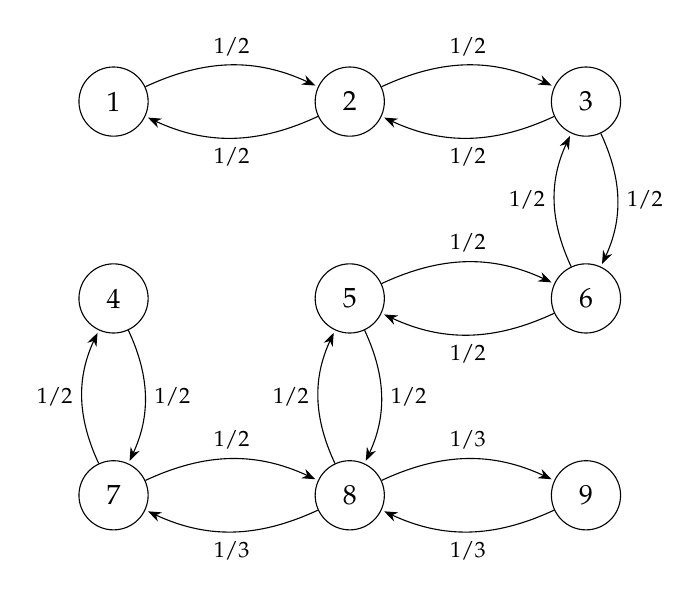
\begin{tikzpicture}[shorten >=1pt,node distance=2.5cm and 3cm,on grid,auto]
\node[state] (q1)               {$1$};
\node[state] (q2) [right=of q1] {$2$};
\node[state] (q3) [right=of q2] {$3$};
\node[state] (q4) [below=of q1] {$4$};
\node[state] (q5) [right=of q4] {$5$};
\node[state] (q6) [right=of q5] {$6$};
\node[state] (q7) [below=of q4] {$7$};
\node[state] (q8) [right=of q7] {$8$};
\node[state] (q9) [right=of q8] {$9$};
\path[->,every node/.style={font=\footnotesize}] 
  (q1) edge[bend left=25] node {1/2} (q2)
  (q2) edge[bend left=25] node {1/2} (q1)
  (q2) edge[bend left=25] node {1/2} (q3)
  (q3) edge[bend left=25] node {1/2} (q2)
  (q3) edge[bend left=25] node {1/2} (q6)
  (q6) edge[bend left=25] node {1/2} (q3)
  (q6) edge[bend left=25] node {1/2} (q5)
  (q5) edge[bend left=25] node {1/2} (q6)
  (q5) edge[bend left=25] node {1/2} (q8)
  (q8) edge[bend left=25] node {1/2} (q5)
  (q4) edge[bend left=25] node {1/2} (q7)
  (q7) edge[bend left=25] node {1/2} (q4)
  (q7) edge[bend left=25] node {1/2} (q8)
  (q8) edge[bend left=25] node {1/3} (q7)
  (q8) edge[bend left=25] node {1/3} (q9)
  (q9) edge[bend left=25] node {1/3} (q8);
\end{tikzpicture}
\end{center}
Privault \cite[Sections~5.3]{privault} computes the expected number of returns to state $0$ starting in any other state and the average number of steps in the simulation is very close to to the expected number of returns:
\begin{verbatim}
Expected steps to return to 0 = [16, 15, 28, 59, 48, 39, 58, 55, 56]
Average  steps to return to 0 = [14, 15, 28, 59, 46, 39, 59, 55, 54]
\end{verbatim}
The simulation of the average number of returns to any state $i$ from any state $j$ gives:
\begin{verbatim}
Average  steps to return to 0 = [14, 15, 28, 59, 46, 39, 59, 55, 54]
Average  steps to return to 1 = [ 1,  8, 14, 43, 31, 24, 42, 40, 40]
Average  steps to return to 2 = [ 3,  2,  8, 31, 20, 10, 29, 27, 30]
Average  steps to return to 3 = [52, 53, 50, 15, 37, 44, 14, 29, 28]
Average  steps to return to 5 = [ 8,  8,  5, 20,  8,  7, 18, 15, 16]
Average  steps to return to 6 = [37, 37, 35,  1, 21, 29,  8, 13, 14]
Average  steps to return to 7 = [25, 23, 21,  4,  9, 16,  3,  5,  1]
Average  steps to return to 8 = [38, 37, 37, 19, 25, 30, 18, 14, 16]
\end{verbatim}
Privault \cite[Sections~7.2]{privault} also computes the expected number of returns to state $i$ from state $i$ and the averages (the main diagonal of the above matrix) are very close:
\begin{verbatim}
Expected steps to return to i from i = [16,  8,  8, 16,  8,  8,  8,  5, 16]
Average  steps to return to i from i = [14,  8,  8, 15,  7,  7,  8,  5, 16]
\end{verbatim}


%%%%%%%%%%%%%%%%%%%%%%%%%%%%%%%%%%%%%%%%%%%%%%%%%%%%%%%%%%%%%%%%%%%%%

\section{Stationary distribution}\label{stationary}

Let $\pi$ be a probability distribution of the initial state of a Markov chain. Take one step according to the transition matrix. If the probability distribution is still $\pi$, it is the \emph{stationary distribution} of the chain. Clearly, the distribution will remain the same no matter how many steps are taken.

For each step in the simulation the initial state is randomly selected according to the distribution and then the transition matrix is used to compute the next state. A count of the these states is maintained and used to obtain a simulated distribution.

Privault \cite[Sections~7.2]{privault} computes the stationary distribution of the maze and the result of the simulation is very close:
\begin{verbatim}
Stationary distribution:
[0.0625, 0.1250, 0.1250, 0.0625, 0.1250, 0.1250, 0.1250, 0.1875, 0.0625]
Distribution after first step:
[0.0626, 0.1277, 0.1269, 0.0612, 0.1248, 0.1261, 0.1240, 0.1883, 0.0584]\end{verbatim}

%%%%%%%%%%%%%%%%%%%%%%%%%%%%%%%%%%%%%%%%%%%%%%%%%%%%%%%%%%%%%%%%%%%%%

\addcontentsline{toc}{section}{References}

\bibliographystyle{plain}
\bibliography{markov}

%%%%%%%%%%%%%%%%%%%%%%%%%%%%%%%%%%%%%%%%%%%%%%%%%%%%%%%%%%%%%%%%%%%%%

\end{document}
